\documentclass[final, 11pt]{article}

\usepackage[italian]{babel}
\usepackage{braket}
\usepackage{diagbox} 
%\usepackage{setspace}
\usepackage{tikz}

\usepackage{amsmath}
\usepackage{amsfonts}
\usepackage{algorithm}		%pseudocodice package
\usepackage{algorithmic}	%pseudocodice package

\usepackage[utf8]{inputenc}

\usepackage{listings}
\usepackage{xcolor}


\usepackage{graphicx}
\usepackage{pdfpages}
\title{Studio di framework per la generazione di fake images di vestiti: Analisi e confronto dei codici VITON e Virtual Try-On with Detail Carving}
\author{ Candidato: Fabio Tarocco VR421748}
\begin{document}
	\clearpage
	
\begin{titlepage}
	\centering
	\vspace*{\fill}
	{\scshape\LARGE Università degli Studi di Verona \par}
	\vspace{1.5cm}
	{\huge Studio di framework per la generazione di fake images di vestiti: Analisi e confronto dei codici VITON e Virtual Try-On with Detail Carving \par}
	\vspace{0.5cm}
	{\scshape  Corso di Laurea Triennale in Informatica \par}
	\vspace{1cm}
	{\Large\itshape Fabio Tarocco VR421748 \par}
	\vspace{1cm}
	\vspace{5cm}
	\vspace*{\fill}
	{\large 16 Ottobre 2020 \par}
\end{titlepage}
	\newpage
	\thispagestyle{plain} % empty
	\mbox{}
	\clearpage
	
	\tableofcontents
	\newpage
	\section{Introduzione al report}
	\subsection{Idea di base}
	La proposta iniziale di stage era quella di analizzare alcuni framework per il riconoscimento dai FAKE images attraverso l’utilizzo di NN e Deep Learning. L’idea era alquanto interessante.
	Per procedere con l’esperienza si è deciso di andare a capire il funzionamento di quello che c’è a monte delle FAKE-IMAGES, cioè la loro creazione.
	
	Si è passati quindi ad un progetto che andasse a studiare il funzionamento e la qualità dei risultati di Frame Work per i virtual Try-On (VTO). La generazione, quindi, di immagini false, artefatte, create attraverso l’utilizzo di codice basato su Reti neurali e Machine Learning, ad hoc per l’ambito della moda e non solo.\\
	Il punto di partenza è stato il codice VITON (portato al CVPR 2018). Una rete per il try-on virtuale image-based, il quale sarà la base di confronto per gli altri codici analizzati durante l’esperienza.
	Proseguendo poi al ricercare un concorrente, sempre basato su VITON, per permettere dei confronti prestazionali. Nell'analisi è stato utilizzato Virtual Try-on with Detail Carving (VTODC). Framework portato al CVPR 2019 e realizzato dalla JDAI CV, con sede a Pechino, che introduce la possibilità di scegliere anche con quale posa generare il modello finale, oltre all’abito e al soggetto.
	
	Infine si è deciso di produrre una demo che permettesse di scegliere una combinazione di soggetti/abiti da un dataset limitato ed eseguire la sostituzione del vestiario con l’opzione di poter introdurre modifiche riguardanti la suddivisione fra i vari segmenti che compongono soggetto di base: vestito, braccia/maniche, pantaloni, viso e capelli.
	
	\subsection {Obiettivi tirocinio}
	L'obbiettivo che ci si è posti come cardine dell'esperienza di tirocinio è stato quello di valutare i risultati, quindi le prestazioni, di più codici che eseguono virtual try-on con base (VITON).
	
	Le richieste erano quelle di capire quando i due codici confrontati producevano output validi e quando invece presentavano difficoltà nel produrli.
	Si è quindi proceduto ad analizzare diversi codici basati sul predecessore VITON e scegliere quelli che potevano avere incrementi sostanziali e visibili nelle prestazioni e nella qualità/affidabilità dei risultati.
	
	Durante l'esperienza si è inoltre deciso di provare ad aggiungere ulteriori obiettivi ossia: Produrre un piccolo applicativo "CANVAS" che permettesse la modifica del label (suddivisione delle componenti del soggetto finale: viso, vestito, braccia, pantaloni, capelli) e applicarlo poi ad una demo "PyTryOn" che permettesse ad un utente di generare differenti outfit, attraverso l'utilizzo di un dataset di campioni ridotto, potendo inoltre utilizzare CANVAS per modificare alcune caratteristiche degli abiti/soggetto.
	
	
	
	\subsection{Cos'è un Virtual Try-On}
	Partiamo spiegando cos'è un virtual try-on. 
	
	È una modalità alternativa con la quale un futuro cliente di un negozio di abbigliamento o di gioielli potrà provare i prodotti dei negozi in modo virtuale, senza dover fisicamente provarli in camerino. Quindi attraverso l'utilizzo di un dispositivo dotato di fotocamera, l'utente può valutare se comprare o meno un capo provandolo virtualmente, attraverso l'utilizzo di realtà aumentata.
	
	Questo approccio, già presente da anni sul mercato ma migliorato mediante l'utilizzo di machine learning
e modelling 3D, permette di provare un capo prima di acquistarlo in qualsiasi luogo, senza l'"obbligo" di andare in negozio, di provare contemporaneamente più capi, valutando anche i vari outfit e soprattutto è time-saving.
	
	Nel caso preso in esame si è operato su codici che prevedevano l'utilizzo di dataset di immagini prese da
un catalogo di abbigliamento di un negozio di e-commerce, quindi non attraverso l'utilizzo di modelling 3D e risultati real-time applicati su video, ma sulla creazione di outfit alternativi a quelli originali utilizzando le coppie modello target e vestito target.
	
	\begin{figure}[!htb]
		\begin{center}
			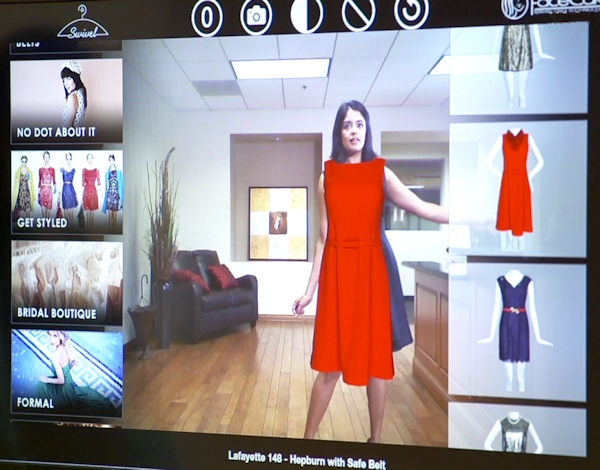
\includegraphics[scale=.7]{FaceCake-virtual-dressing-room.jpg}
		\end{center} \caption{Dressing room dotata di VTO in real time}
	\end{figure} 

	\section{VITON}
	\subsection{Cos'è VITON}
	È un Virtual Try-On Image-Based realizzato e pubblicato da alcuni ricercatori/studenti dell’Università del Maryland. Hanno presentato un codice il quale si pone come obiettivo quello di produrre un’immagine di try-On andando semplicemente ad applicare il vestito (sottoforma di immagine RGB) sul soggetto senza l’ausilio di informazioni provenienti dal 3D. Il codice va quindi a sintetizzare una nuova immagine foto-realistica sovrapponendo un artefatto alla regione corrispondente al vestito del soggetto. 
	
	VITON nasce per risolvere i problemi delle GANs (generative adversarial network, rete generativa avversaria) le quali riescono a produrre ottimi risultati nella generazione delle immagini, traslazioni image-to-image o task di editing, ma hanno difficoltà nella realizzazione di dettagli e deformazioni realistiche di oggetti, in questo caso l’abito target.
	
	Il traguardo di VITON è quello di, prendendo un’immagine di un soggetto vestito come riferimento e un abito target, generare una nuova immagine dove l’abito target è trasferito nel modo più naturale possibile sul soggetto di riferimento.
	
	\subsection{Componenti VITON}
	Il punto più importante durante la realizzazione dell’immagine finale è la generazione dei dettagli/deformazioni che l’abito subisce in base alla posa del soggetto. Viene quindi utilizzato una rappresentazione a 18 keypoints (coordinate su una matrice in formato MicrosoftAccess) per memorizzare le informazioni delle pose di ogni soggetto inserito nel dataset. 
	
	In concomitanza di questo vengono utilizzate anche delle segmentazioni, ottenute mediante un Human Parser, nelle quali si evidenziano le coordinate delle parti del corpo in cui il soggetto è suddiviso. Inoltre, per mantenere l’identità del soggetto, sono state introdotte degli attributi “fisici” come ad esempio faccia, carnagione, taglio di capelli, ecc, i quali saranno poi utilizzati in fase terminale per ricostruire l’immagine finale.
	
	Altra componente importante è l’operazione di Wrapping dell’abito target sul soggetto. Le informazioni necessarie alla realizzazione di un wrap realistico vengono prese direttamente dai dati acquisiti in fase di segmentazione del soggetto. La clothing mask viene utilizzata in fase finale per il riempimento in modo corretto delle zone del soggetto in cui l’abito target dovrà esser visualizzato.
	\newpage
	In tutto questo VITON è suddiviso nel suo funzionamento in 3 componenti:
	\begin{itemize}
		\item Lo stage1 in cui avviene una prima generazione dell’immagine senza dettagli degli abiti;
		\item La run dello script matlab Shape Context Wrap per la realizzazione di un TPS Transfromation dalla quale si ottengono i punti di deformazione del piano;
		\item Lancio dello stage2 (Refinement) in cui grazie ai punti di deformazione ottenuti dallo script matlab vengono applicati i dettagli, trascurati dallo stage1, adattati al vestito.
	\end{itemize}

	\section{VTO con Detail Carving}
	\subsection{Cos'è VTO con Detail Carving}
	Framework multilivello per virtual try-on realizzato da alcuni ricercatori/studenti della Huazhong University of Science and Technology in collaborazione con la JD AI Research di pechino. 
	
	Sfrutta la possibilità di scegliere pose arbitrarie per produrre l’immagine risultante, ma allo stesso tempo cerca di risolvere il problema di mancanza di dettagli degli altri framework per VTO.  VTODC si pone come obbiettivo quello di mantenere caratteristiche del volto, dell’età e soprattutto dettagli dell’abito pur riuscendo a mantenere un fitting dell’abito target il più realistico possibile. 
	
	Il focus principale per il quale è stato realizzato VTODC è quello di andare incontro alle esigenze dei clienti che, non solo vorrebbero provare un abito, ma vedere come quest’ultimo calza in differenti pose e il più realisticamente possibile.
	
	A differenza di VITON, VTODC necessita di input diversi dal dataset per poter operare, infatti, non solo chiede segmentazione del soggetto, cloth map e immagini target abito e soggetto, ma richiede la colormap di come  il soggetto è suddiviso in parti e i keypoints delle pose target, in formato json e non più Microsoft Access Table. Il codice inoltre, non è più suddiviso nell’esecuzione di tre parti differenti, bensì ne viene lanciato uno solo, ossia il file “demo.py”. 
	
	\newpage
	\section{Confronto risultati fra i due framework}
	\subsection{Output VITON}
	Come da richiesta, durante l'esperienza di tirocinio si è dovuto trovare una buona base di confronto per capire il miglioramento/lacune di altri codici per VTO.\\Per fare ciò è stato necessario eseguire più volte il codice VITON per aumentare la pool di campion da confrontare e per capire i limiti dello stesso.\\
	È stato inoltre deciso che il livello di train in cui si trovava VITON al momento del pull da GitHub dalla repository iniziale fosse sufficiente per ottenere dei risultati accettabili sui quali eseguire poi i confronti con il codice Virtual Try-On with Detail Carving (VTODC).\\
	
	I risultati vengo salvati sottoforma di concatenazione di 7 immagini: modello target, abito target, wrap dell'abito target sul soggetto target, risultato stage1, cloth mask dello stage1, risultato finale ossia stage2 (post refinement) e relativa cloth mask.
	
	\begin{figure}[!htb]
		\centering
		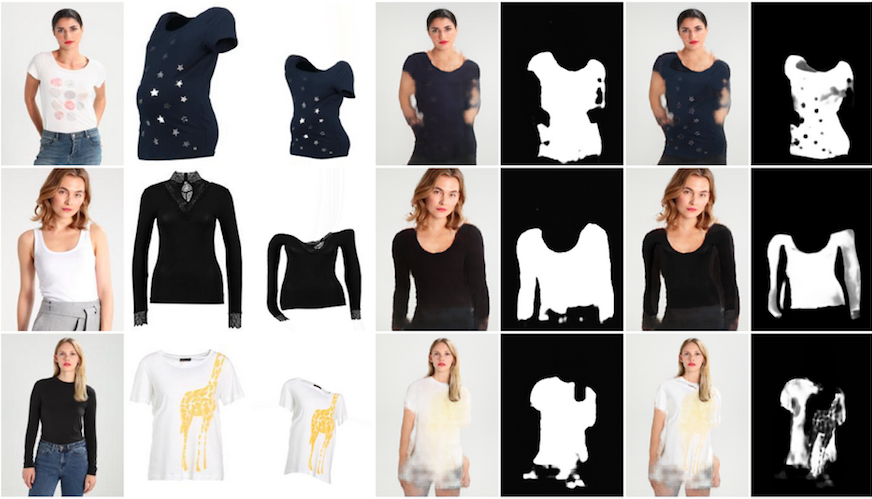
\includegraphics[width=\linewidth]{vitonres1_1.png}
		\caption{Alcuni degli output generati}
	\end{figure} 
	
	\subsection{Output VTODC}
	Per quanto riguarda la parte di VTODC, come già spiegato nella parte di introduzione al codice, si è cercato di utilizzare lo stesso dataset di VITON, ma non avendo la possibilità di eseguire segmentazione in modo indipendente e non avendo tutti gli input necessari per il funzionamento corretto del codice, si è deciso di utilizzare il dataset fornito nella repository, anche se molto limitato.
	
	L’immagine risultato è la concatenazione di 8 immagini: Soggetto target, abito target, posa target, wrap dell’abito sul modello sulla posa target, colormap della suddivisione del soggetto target, nuova colormap della segmentazione del soggetto con posa target, risultato pre-refinement, immagine risultante con miglioramento del dettaglio.
	
	\begin{figure}[!htb]
		\centering
		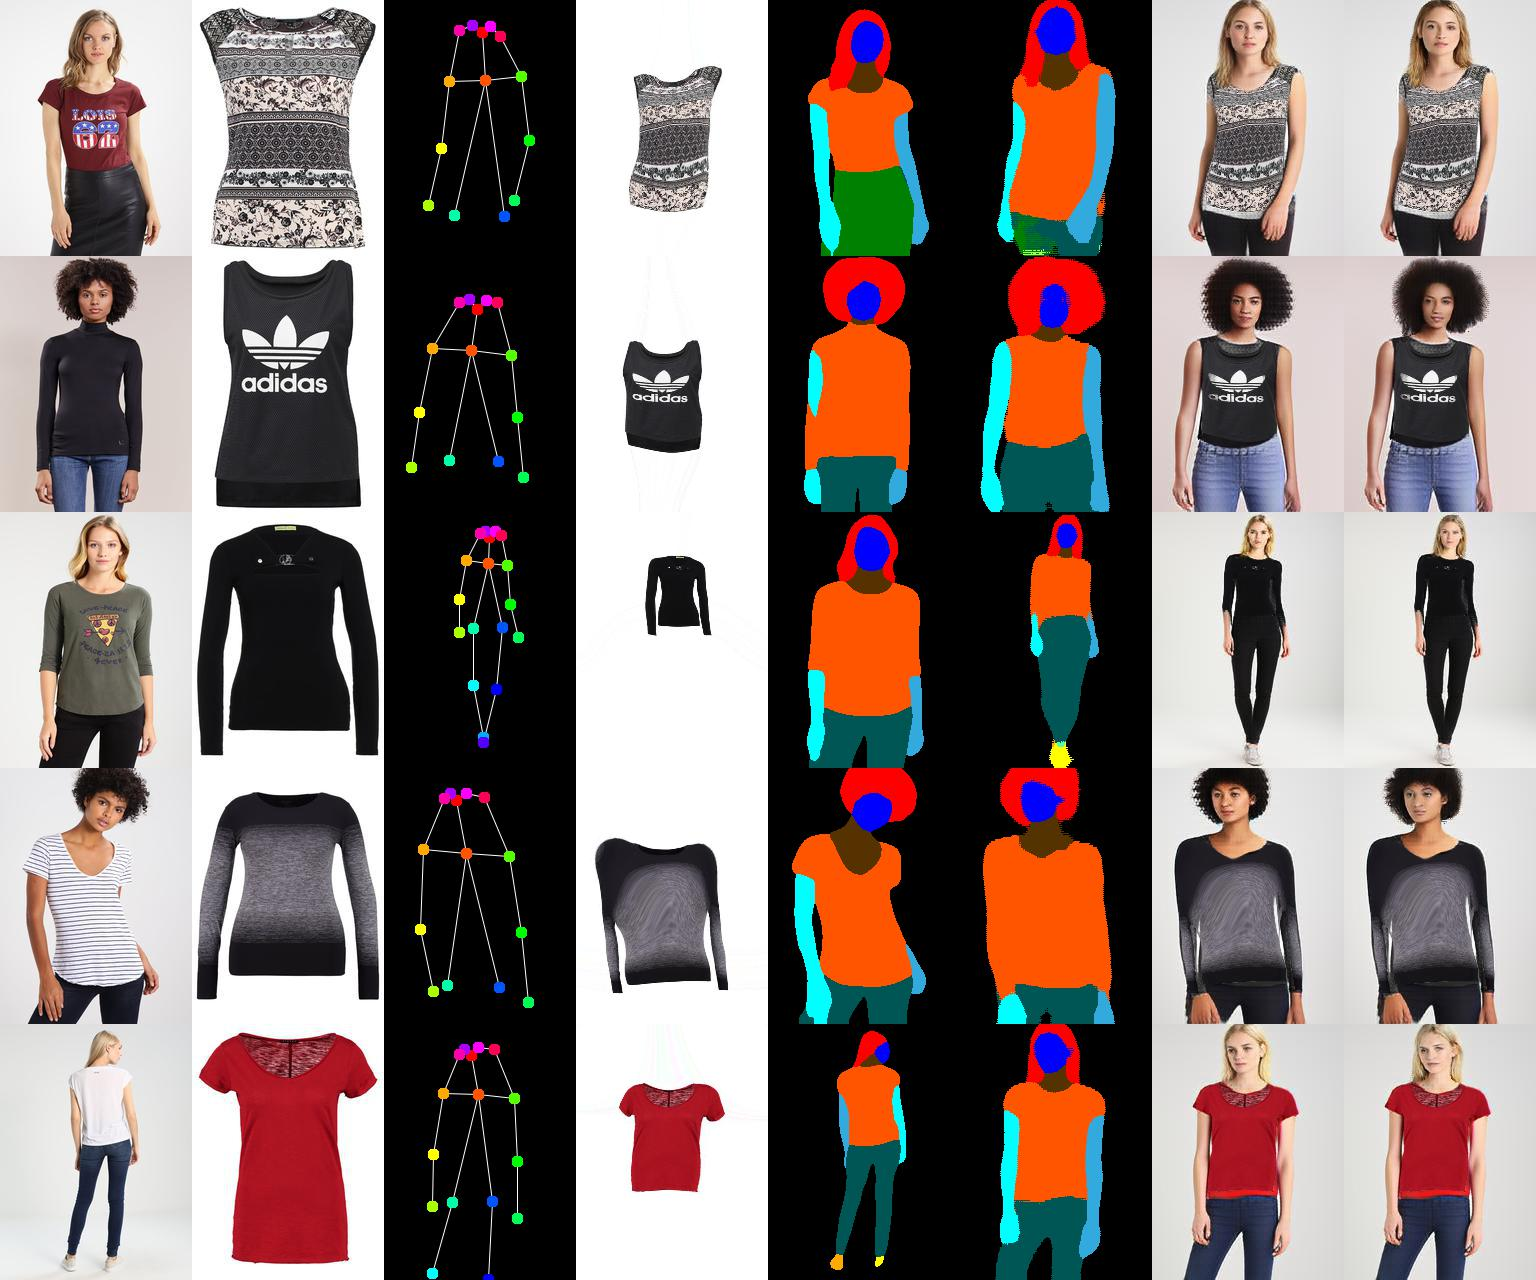
\includegraphics[width=\linewidth]{Detailcarvingresult.jpg}
		\caption{Immagini di output}
	\end{figure} 
	
	\subsection{Codici a confronto}
	Mettendo a confronto i risultati dei due codici si possono trarre le seguenti conclusioni, il  tutto ricordandosi che, non potendo effettuare training su entrambi i codici ci si è basati sui risultati ottenuti con meno ore di train rispetto a quelle con cui sono stati realizzati i paper pubblicati.
	
	\begin{itemize}
		\item I risultati ottenuti mediante l'utilizzo di VTODC sono molto dettagliati: rappresenta in modo chiaro il pattern nel caso in cui il vestito ne sia fornito e mantiene le caratteristiche facciali del soggetto.
		\item 	Nel caso di VITON notiamo della difficoltà nel definire in modo chiaro la posizione e conformazione degli arti, sia nel dettaglio (dita) e non (delineamento delle braccia). Questo però accade nel momento in cui si deve ricostruire parte o tutto l’arto da un’immagine di partenza in cui il soggetto presentava maniche lunghe e come abito target si ha una maglia a maniche corte/smanicato.
		Il concorrente VTODC, invece, riesce in modo più che chiaro a definire sia l’arto e sia le dita del soggetto, in entrambi i casi: partendo da maniche lunghe per passare a corte e viceversa.
		\begin{figure}[!htb]
			\centering
			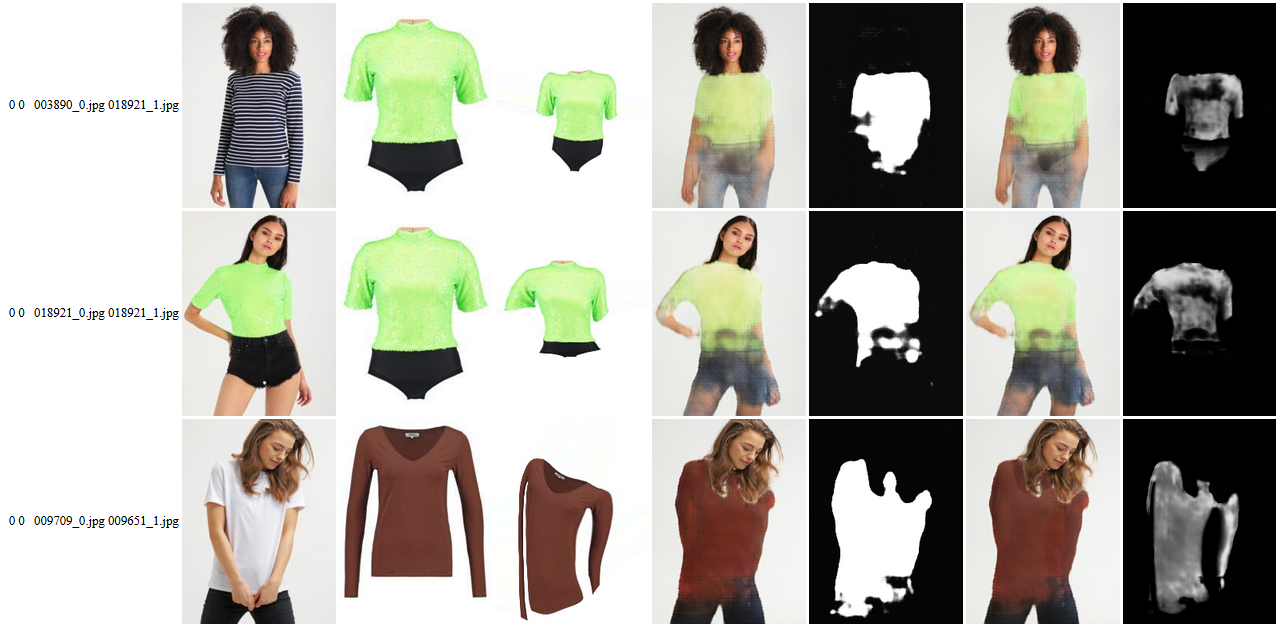
\includegraphics[width=\linewidth]{viton_err_2.png}
			\caption{Notare come gli arti vengano fusi con l'abito}
		\end{figure} 
		\item	VITON presenta difficolta con soggetti che non sono posizionati in modo frontale all’obbiettivo della fotocamera, ad esempio di spalle o laterali, oppure con figure che appaiono nell’immagine dalla cinta in giù e non solamente vita/busto. 
		
		\begin{figure}[!htb]
			\centering
			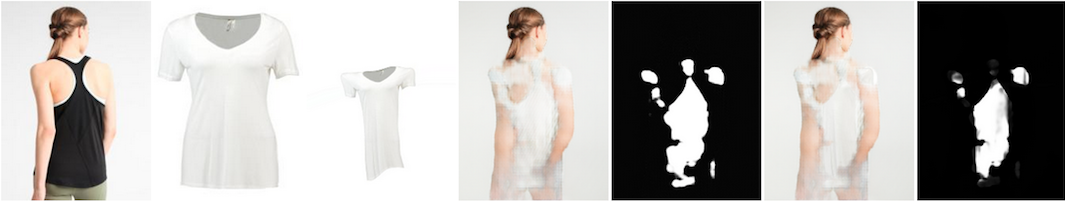
\includegraphics[width=\linewidth]{spalleviton.png}
			\caption{Evidente difficolta nell'identificare la posa}
		\end{figure} 
		\item	Il problema sopra citato è invece risolto con l’utilizzo di VTODC grazie all’utilizzo di una target pose, cosa che in VITON non era presente.
		Non solo si possono utilizzare soggetti di spalle, ma anche permette di cambiare completamente la posa di un soggetto.
		
		\begin{figure}[!htb]
			\centering
			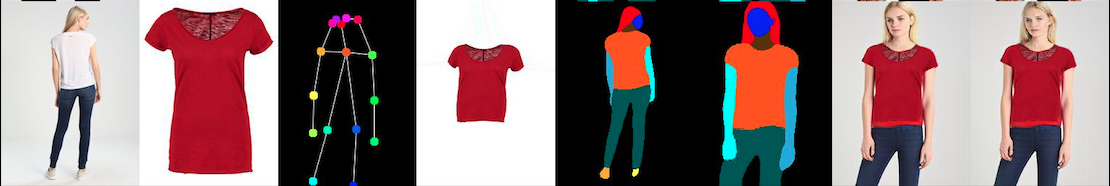
\includegraphics[width=\linewidth]{scollaturaDC.png}
			\caption{Soggetto di spalle ricostruito in posa frontale}
		\end{figure} 
	
		\item Abiti dettagliati, abiti con fantasie/pattern o con scritte, vengono difficilmente trasportati da VITON sull’immagine risultato. Quello che viene prodotto è un miscuglio non ben definito dell’immagine dell’abito e del colore di base, ottenuto del riempimento all’interno della cloth map effettuato dal codice nella fase preliminare.\\
		Ad esempio: La presenza di fasce o scritte sulla maglietta, l’algoritmo le ignora coprendole con il colore dominante della maglietta.
		\begin{figure}[!htb]
			\centering
			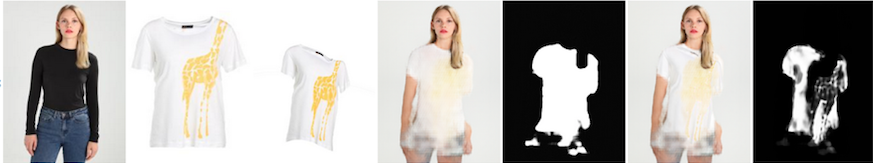
\includegraphics[width=\linewidth]{dettaglioV.png}
			\caption{Stampa sulla maglietta sfumata con l'abito}
		\end{figure} \newpage
		\item 	Con VITON se il soggetto ha le mani o gli arti sopra il vestiario, l’algoritmo le considera come parte di quest’ultimo, provvedendo a colorarli della stessa tinta.
		
		\begin{figure}[!htb]
			\centering
			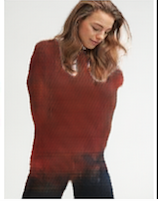
\includegraphics[width=.2\linewidth]{nomani.png}
			\caption{Funsione completa degli arti con l'abito}
		\end{figure} 
		
	\end{itemize}
	
	
	Si capisce quindi che, con il livello di training utilizzato per effettuare i test, la versione con Detail Carving produce dei risultati notevolmente migliori rispetto al concorrente VITON.
	Inoltre, sarebbe stato interessante effettuare alcuni cicli di train per migliorare i risultati di VITON, in modo tale da verificare o meno le stesse capacità di produzione di immagini artefatte di VTODC, in contemporanea sarebbe risultato ancora più chiaro il confronto se entrambi i codici avessero operato sullo stesso dataset.
	\newpage
	
	\section{Demo PyTryOn: applicazione di ACGPN}
	\subsection{Introduzione alla Demo}
	L’applicativo che si è deciso di produrre doveva soddisfare due requisiti principali:
	\begin{itemize}
		\item Permettere all’utente la possibilità di scegliere la coppia Modello-Abito
		\item Modifica delle segmentazioni relative alle componenti che formavano l’immagine di base:
		Ciano= capelli, Violetto = viso, Azzurro = Abito, Giallo = Pantaloni, Arancio/Rosso = Braccio DX
		Verde = Braccio SX
	\end{itemize}

	\begin{figure}[!htb]
		\begin{center}
			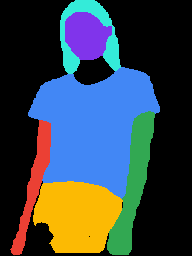
\includegraphics[scale=.7]{002474_0.png}
		\end{center} \caption{Schema colore della suddivione addottata nei Label da ACGPN}
	\end{figure} 
	
	È stato scelto come Framework per la sostituzione dell’abito il sorgente ACGPN, portato all’CVPR nell’edizione 2020. 
	Sistema realizzato nell’ambiente di sviluppo CUDA ossia l'architettura hardware creata da NVIDIA per consentire l’elaborazione parallela. Per eseguire questo codice è stato necessario l’utilizzo di macchine più performanti ed è stato possibile grazie all’accesso alle macchine dell’Università di Verona, su cui si è lavorato tramite SSH.
	
	
	PyTryOn è formato da due componenti principali: la prima è il wrapper che contiene CANVAS (app per la modifica dei label) e lo script per la selezione delle immagini sorgenti dal dataset di cui è dotato il programma, la seconda invece, è l’eseguibile test.py contenuto nella sezione di ACGPN dedicata alle fasi di testing, ossia quella di Inference.
	
	Tralasciando le parti già presenti nella repository iniziale di ACGPN, il codice è stato scritto completamente in Python. Il codice di PyTryOn è poi stato portato all’interno dell’ambiente di lavoro di ACPGN in modo da aver accesso diretto a test.py e soprattutto al Dataset.
	
	Per quanto riguarda quest’ultima componente, il dataset utilizzato nella demo prodotta è un sottoinsieme di quello utilizzato per ACGPN e VITON. Per le fasi di test e debugging si è optato per un dataset della dimensione di 5 modelli e 5 abiti scelti in modo casuale da quello originale, selezionando quelle immagini che non portassero a problemi di Missing keypoints o deformazioni varie nel risultato (stessi problemi riscontrati nei test di VITON).
	
	\subsection{Descrizione interfaccia}
	Quello che l’utente si trova davanti è un’interfaccia minimale e alquanto spartana, non era necessario aggiungere tanti dettagli, ma rendere il più possibile leggero l’applicativo dovendolo eseguire via SSH.
	
	\begin{figure}[!htb]
		\centering
		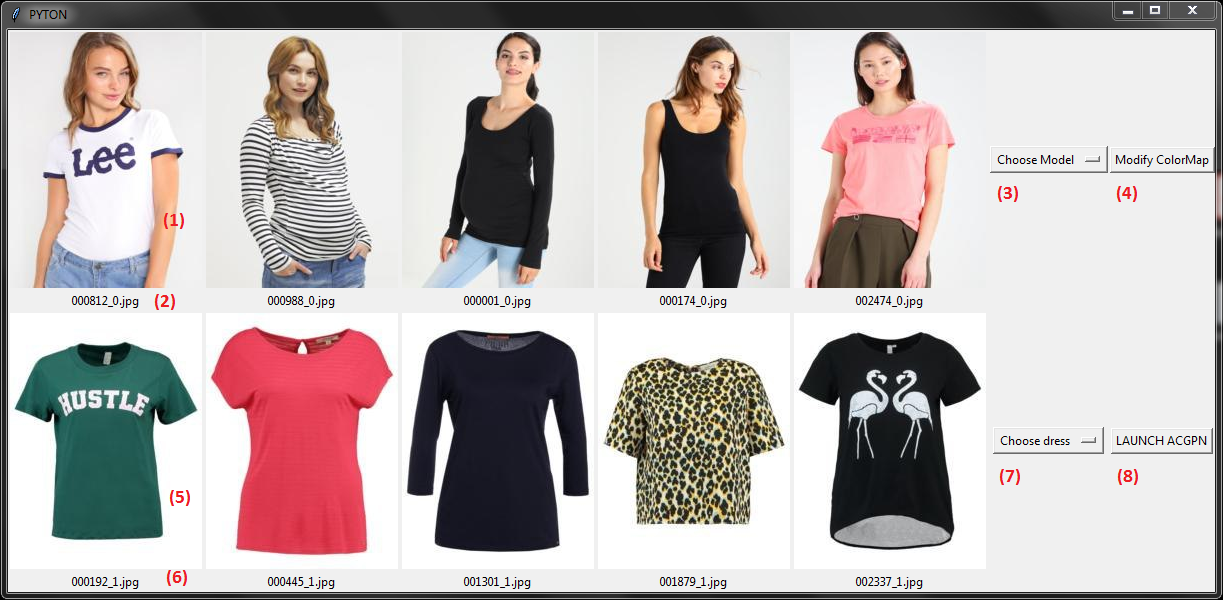
\includegraphics[width=\linewidth]{PyTryOn_numerata_1.png}
		\caption{Interfaccia principale}
	\end{figure} 

L’interfaccia è così suddivisa:\\
	(1) Anteprima dei Soggetti utilizzabili come base per il VTO.
\\
	(2) Relative codifiche delle immagini dei soggetti.
\\
	(3) Menu a tendina per la selezione del soggetto. 
\\
	(4) Tasto avviare l’applicativo per la modifica delle suddivisioni del soggetto. 
\\
	(5) Anteprima degli Abiti utilizzabili come target per il VTO. 
\\
	(6) Come sopra, relative codifiche delle immagini degli abiti. \\
	(7) Menu a tendina per la selezione degli abiti.
\\
	(8) Avvio del file di test.py per la produzione del risultato. 
\\
	
	\begin{figure}[!htb]
		\centering
		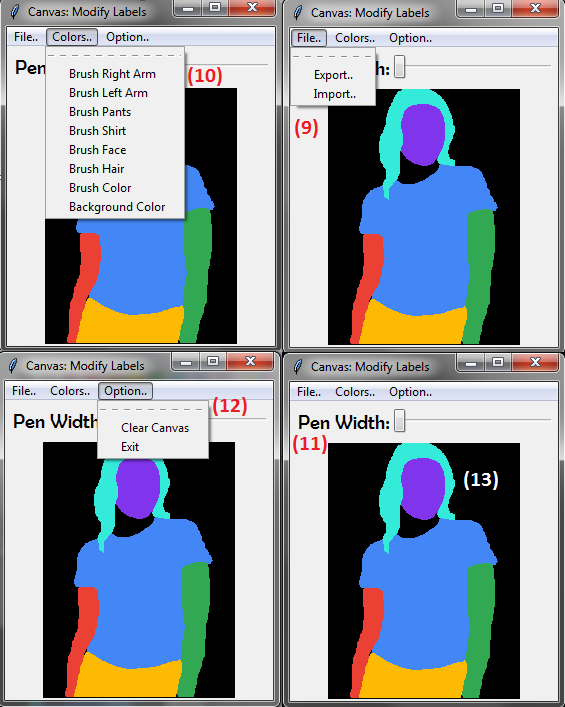
\includegraphics[width=0.5\linewidth]{PyTryOn_numerata_2.png}
		\caption{Interfaccia applicazione Canvas}
	\end{figure} 
	Passando all’interfaccia della mini applicazione per la modifica delle segmentazioni “CANVAS” abbiamo:
\newline
	(9) Menù a tendina per la selezione di import/export dell’immagine da modificare. \\
	(10) Menu a tendina per la selezione del colore del pennello in base alla parte della segmentazione che si vuole modificare. 
\\
	(11) Cursore per la selezione della dimensione del pennello. 
\\
	(12) Tasto reset, per rimuovere l’immagine che si stava modificando. \\
	(13) Piano di disegno su cui si può modificare l’immagine sorgente.
\\
	
	\subsection{Funzionamento}
	La componente principale che ci permette di modificare le segmentazioni in cui il modello è suddiviso in modo chiaro e intuitivo è resa possibile grazie all’utilizzo di uno script di conversione da Grey Scale a RGB seguendo gli assegnamenti che sono stati scelti dagli sviluppatori di ACGPN. 
	
	Nel momento in cui si va a selezionare una delle immagini che si vuole modificare, viene effettuata la conversione e aperta sulla tavola, viceversa, quando si va ad effettuare il salvataggio si passa da RGB a GreyScale. Per effettuare questa conversione abbiamo utilizzato un due cicli annidati e tenendo conto delle varie codifica/valori che ogni pixel assumeva, si andava a sostituire con il codice coloro corrispondente alla controparte convertita.
	
	Questo applicativo è stato creato utilizzando i pacchetti TKINTER e PILLOW, il primo per generare GUI su Python mentre il secondo utilizzato ogniqualvolta si devono manipolare immagini, aprirle o salvarle.
	Utilizzando questi pacchetti è stata generata anche l’interfaccia e il codice dell’applicativo principale “DEMO\_PyTryOn”, ossia quello che racchiude CANVAS e il test.py per il lancio del VTO.
	
	In questa parte non c’è nulla di articolato, viene data la possibilità all’utente di scegliere l’outfit e il soggetto mediante l’utilizzo di due menu a tendina con i relativi codici dei campioni proposti ed inoltre è presente il tasto per l’avvio di CANVAS.
	
	L’altro tasto presente nell’interfaccia principale (4) è quello per l’avvio del virtual try-on, quindi dello script per il testing di ACGPN.
	Il sistema di ACGPN utilizza input diversi rispetto alle due alternative proposte in precedenza: VITON e VTODC, infatti richiede:
	\begin{itemize}
		\item Abito target
		\item Modello di base
		\item Label del modello in grayscale
		\item Edge degli abiti
		\item Keypoints del soggetto in formato json
	\end{itemize}
	Durante l’utilizzo dell’applicativo è possibile modificare 3 dei 5 punti utilizzati come input, ossia i primi 3.
	
	\subsection{Risultati}
	Quello che è stato ottenuto dai vari testing della demo è un risultato non molto eclatante, infatti, ACGPN sembra ignorare in gran parte le modifiche che vengono applicate sul label di input, il quale viene sostituito, in fase di ricostruzione del risultato finale, con uno generato dal codice.
	Il label che si va a modificare viene preso in considerazione in modo marginale, viene anzi, effettuate delle modifiche ulteriori su di esso per migliorare la resa dell’abito target sul soggetto target, tendendo conto delle condizioni iniziali e finali a cui si vuole arrivare. 
	Queste possono essere suddivise in 3 alternative:
	\begin{enumerate}
		\item Il soggetto iniziale presenta un abito a maniche lunghe mentre l’abito target è a maniche corte, comporta la mancanza di riferimenti per la ricostruzione delle braccia scoperte e per risolvere questo interviene ACGPN sovrascrivendo le modifiche manualmente eseguite con CANVAS.
		\item Il soggetto target presente un abito a maniche corte mentre l’abito d’arrivo è a maniche lunghe, semplicemente avviene una sovrapposizione, seguendo il wrapping corretto, dell’abito sul soggetto, ignorando eventuali modifiche.
		\item Il vestito target è più corto di quello del soggetto target. In questo caso il risultato che si ottiene e simile a quelli ottenuti con VITON, quindi una fusione fra abito e pantalone a chiazze.
	\end{enumerate}
	
	
	\begin{figure}[!htb]
		\centering
		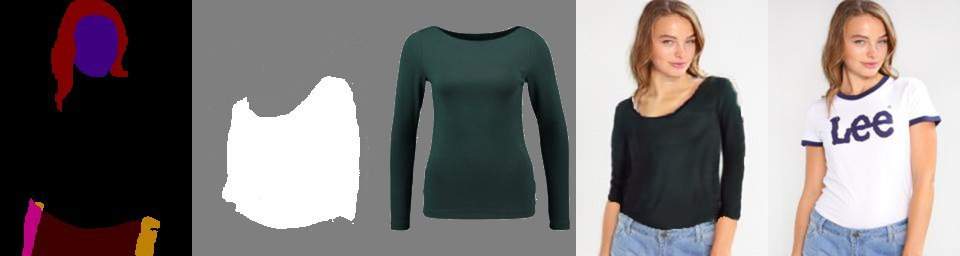
\includegraphics[width=0.7\linewidth]{demo2.jpg}
		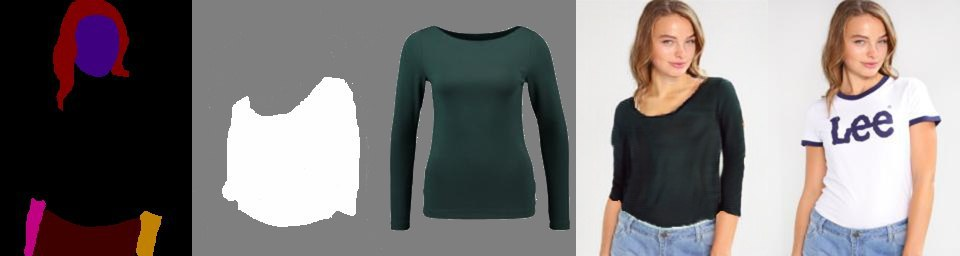
\includegraphics[width=0.7\linewidth]{demo2_b.jpg}
		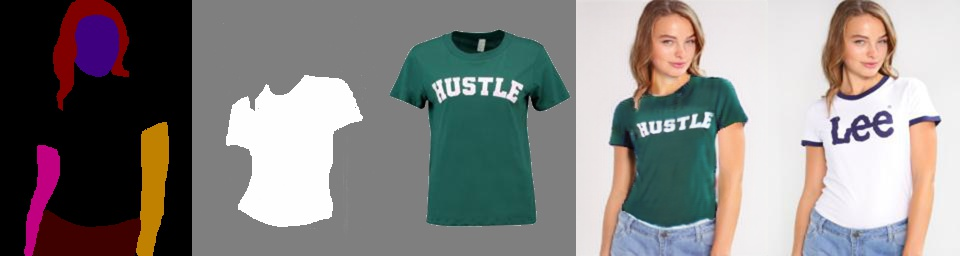
\includegraphics[width=0.7\linewidth]{OtherRes.jpg}
		\caption{ILa prima immagine senza utilizzo di Cavas, la seconda con la modifica del label}
	\end{figure} 


	
\end{document}